\documentclass[11pt]{article}

\usepackage[a4paper,margin=25mm,headheight=15pt]{geometry}
\usepackage[T1]{fontenc}
\usepackage[utf8]{inputenc}
\usepackage{lmodern}
\usepackage{microtype}
\usepackage{amsmath,amssymb,amsthm,mathtools}
\usepackage{booktabs,longtable,tabularx,array,multirow}
\usepackage{enumitem}
\usepackage{xcolor}
\usepackage{graphicx}
\usepackage{tikz}
\usetikzlibrary{arrows.meta,positioning,fit,calc,shapes.geometric}
\usepackage{listings}
\usepackage{caption}
\usepackage{subcaption}
\usepackage{float}
\usepackage{fancyhdr}
\usepackage{url}
\usepackage[colorlinks=true,linkcolor=blue!55!black,citecolor=green!40!black,urlcolor=blue!60!black]{hyperref}
\hypersetup{
  pdftitle={CBSC-ZDC: An Auditable Specification for a Four-Momentum-Conditioned Fast Monte Carlo Surrogate},
  pdfauthor={ASIoP ZDC FastMC Project},
  pdfsubject={Mathematical research plan, implementation contract, and falsifiable comparison protocol for neutron ZDC FastMC},
  pdfkeywords={Fast Monte Carlo, Zero Degree Calorimeter, neutron, Geant4, conditional flow matching, sparse generation}
}
\usepackage[nameinlink,noabbrev]{cleveref}
\usepackage[backend=biber,style=numeric,sorting=none,natbib=true,maxbibnames=8]{biblatex}
\addbibresource{references.bib}

\definecolor{deepblue}{RGB}{18,57,92}
\definecolor{lightblue}{RGB}{230,240,248}
\definecolor{lightgray}{RGB}{246,246,246}
\definecolor{deepred}{RGB}{130,28,28}
\definecolor{deepgreen}{RGB}{26,105,64}

\pagestyle{fancy}
\fancyhf{}
\lhead{CBSC-ZDC Auditor Specification}
\rhead{Research design, not a fidelity claim}
\cfoot{\thepage}

\newtheorem{proposition}{Proposition}[section]
\newtheorem{theorem}[proposition]{Theorem}
\newtheorem{lemma}[proposition]{Lemma}
\newtheorem{corollary}[proposition]{Corollary}
\theoremstyle{definition}
\newtheorem{definition}[proposition]{Definition}
\newtheorem{assumption}[proposition]{Assumption}
\theoremstyle{remark}
\newtheorem{remark}[proposition]{Remark}

\newcommand{\pG}{p_{\mathrm{G4}}}
\newcommand{\pM}{p_{\theta}}
\newcommand{\R}{\mathbb{R}}
\newcommand{\E}{\mathbb{E}}
\newcommand{\G}{\mathcal{G}}
\newcommand{\given}{\,\vert\,}
\newcommand{\ind}{\mathbf{1}}
\newcommand{\softmax}{\operatorname{softmax}}
\newcommand{\sigmoid}{\operatorname{sigmoid}}
\newcommand{\logit}{\operatorname{logit}}
\newcommand{\Cat}{\operatorname{Cat}}
\newcommand{\Bern}{\operatorname{Bern}}
\newcommand{\BetaDist}{\operatorname{Beta}}
\newcommand{\GeV}{\,\mathrm{GeV}}
\newcommand{\code}[1]{\texttt{#1}}

\lstset{
  basicstyle=\ttfamily\small,
  backgroundcolor=\color{lightgray},
  frame=single,
  breaklines=true,
  columns=fullflexible,
  keepspaces=true,
  showstringspaces=false
}

\title{\textbf{CBSC-ZDC: An Auditable Specification for a Four-Momentum-Conditioned Fast Monte Carlo Surrogate of Neutron Showers in a Zero Degree Calorimeter}\\[0.7em]
\large A mathematical research plan, implementation contract, and falsifiable comparison protocol}
\author{ASIoP ZDC FastMC Project\\Independent research specification}
\date{23 July 2026}

\begin{document}
\maketitle

\begin{abstract}
This document specifies a reproducible research experiment for learning the readout-level distribution of single-neutron Geant4 showers in a fixed Zero Degree Calorimeter (ZDC). The sole raw per-event condition is the incident four-momentum $p^\mu=(E,p_x,p_y,p_z)$; all other event features must be deterministic functions of that vector, while detector geometry is frozen metadata. The proposed model, called the Constrained Budgeted Stochastic Cascade for ZDCs (CBSC-ZDC), is deliberately assembled from established components: a response hurdle, a bounded or target-correct response distribution, a first-visible-layer survival model, an exact-zero longitudinal support model, a masked-simplex energy profile, a finite-support count model, conditional flow matching, edge-conditioned graph message passing, causal layer attention, Gumbel-Top-$k$ support sampling, and exact budget-preserving decoding. No individual component is claimed as a new architecture.

The central correction to the motivating idea is that deposited energy must \emph{not} be forced to decrease from layer to layer. Neutron-induced hadronic showers may begin late, grow, fluctuate, and exhibit secondary maxima. Only the remaining accounting budget is required to be non-increasing. A second central contribution is an exact anti-dust decoder: a generated layer count selects exactly that many cells, all unselected cells are exactly zero, and selected cells receive a threshold floor plus a normalized share of the remaining layer budget. This prevents a model from improving an energy loss by adding a small positive value to every nominally empty cell.

The document is an auditor-ready design specification, not a report of validated physics performance. If the stated data assumptions hold and the implementation follows the mathematical contract, the resulting experiment should be structurally valid and reproducible, with explicit mechanisms and diagnostics designed to prevent or reveal the specific support, energy-accounting, graph, and exposure-bias defects identified in earlier project models. No architecture can guarantee agreement with Geant4 before training and held-out evaluation; that question remains empirical.
\end{abstract}

\vspace{0.5em}
\noindent\colorbox{lightblue}{\parbox{0.96\textwidth}{
\textbf{Assurance statement.} ``Implementing this specification exactly should work'' means that the experiment should be scientifically interpretable and should satisfy the proved algebraic invariants under the stated target assumptions. It does \emph{not} mean that the trained neural distribution is guaranteed to reproduce Geant4 within any numerical tolerance. Fidelity, speed, and usefulness must be measured.
}}

\tableofcontents
\newpage

\section{Scope, status, and precise claim}

\subsection{Research question}
Let $Y\in\R_{\ge 0}^{6790}$ denote the event-level readout vector for one neutron traversing the fixed detector geometry $\G$. The research question is
\begin{equation}
  \text{Can }\pM(Y\given p^\mu,\G)\text{ approximate }\pG(Y\given p^\mu,\G)
\end{equation}
throughout the declared $50$--$250\GeV$ reporting domain, while remaining computationally useful and respecting the exact readout contract?

The available simulation support is described as approximately $0$--$300\GeV$ non-pencil-beam neutron Geant4 data. The broader range may be used for a controlled training-support comparison, but primary results must remain separated from lower- and upper-energy stress regions.

\subsection{What is and is not claimed}
This specification claims the following.
\begin{enumerate}[label=\textbf{C\arabic*.},leftmargin=2.2em]
  \item The original monotone-per-layer-deposit constraint is physically inappropriate for hadronic neutron showers; a monotone remaining budget is the correct conservation structure.
  \item The proposed factorization uses known, published model classes and can be implemented without inventing a new primitive architecture.
  \item Under explicit target assumptions, the decoder guarantees nonnegative cell outputs, exact zeros outside generated support, threshold consistency, and exact accounting identities.
  \item The proposed training and reporting protocol separates implementation validity from empirical detector fidelity.
\end{enumerate}
It does not claim that CBSC-ZDC has already been trained, that it is superior to existing ZDC methods, or that its output is experimentally calibrated detector data. Geant4 itself is a configured stochastic transport simulation whose predictions depend on the detector, materials, production cuts, physics list, and scoring definition \citep{geant4_2003,geant4_2006,geant4_2016,geant4_hadronic_manual}.

\subsection{Relationship to previous project models}
Two prior trained models provide negative evidence and reusable engineering lessons. The legacy recurrent HurdleGraph model exhibited an unbounded total-response tail, positive energy in nominally inactive layers, invalid cross-layer slot correspondence, unused recurrent state, isolated valid graph nodes, and highly separable generated events \citep{project_legacy_audit}. HGF-ZDC was structurally stronger but retained a large response bias, late-HCAL suppression, loss--physics misalignment, weak speed, and an invalid fixed-condition reference construction \citep{project_hgf_audit}. The supplied single-stage graph-flow proposal remains a necessary controlled baseline because it tests whether explicit hierarchy earns its cost on the same data and geometry \citep{project_single_stage}.

\section{Physics basis: neutrons, hadronic showers, ZDCs, and Geant4}

\subsection{Why neutrons make the longitudinal problem stochastic}
A high-energy neutron is electrically neutral and therefore does not continuously ionize like a charged particle before a hadronic interaction. In Geant4, a hadronic process combines cross sections that determine interaction occurrence with final-state models that generate the products; multiple models cover different energy ranges and physical regimes \citep{geant4_hadronic_manual}. Consequently, two neutrons with the same macroscopic four-momentum can have different first visible interaction depths, secondary multiplicities, electromagnetic fractions, nuclear breakup, invisible energy, transverse widths, and leakage.

The average longitudinal profile of a calorimeter shower can often be summarized by smooth parameterizations, including gamma-family forms, but event-level hadronic profiles are neither deterministic nor layerwise monotone \citep{hadronic_profile,gflash}. A neutron may deposit little energy in early material, initiate a cascade later, rise toward a shower maximum, and then decay. Therefore the constraint
\begin{equation}
  D_{\ell+1}\le D_\ell \quad \text{for all layers }\ell
\end{equation}
is rejected. It would make a late-start event impossible: once an early $D_\ell$ is near zero, all subsequent deposits would be forced near zero.

\subsection{Role of a Zero Degree Calorimeter}
ZDCs are forward hadronic calorimeters designed to measure neutral or charged spectator nucleons close to the beam direction. Their response is detector-specific: geometry, segmentation, absorber, active material, acceptance, beam conditions, and readout all shape the observed spectrum and resolution \citep{alice_zdc_tdr,zdc_multinucleon}. Published ALICE ZDC generative work is therefore an important methodological baseline but not a drop-in representation for a detector with 6,790 irregular readout channels \citep{zdcmachinelearning,zdcdiffusion,fasterzdc,expertsim,zdc_iaf}.

\subsection{Why the model should emulate the scored target, not microscopic transport}
The surrogate target is the distribution of stored detector outputs, not an unsupervised reconstruction of Geant4's internal particle history. Learned ``transport,'' ``branching,'' or ``energy flow'' should be interpreted as statistical dependence unless track-level or step-level truth supervises a microscopic claim. The model may incorporate detector depth, adjacency, and remaining budget as inductive biases, but it remains a conditional density estimator for the scored response.

\section{Data contract and supported condition manifold}

\subsection{Sole raw condition}
The public event interface is exactly
\begin{equation}
  p^\mu=(E,p_x,p_y,p_z)\in\R^4.
\end{equation}
For a neutron of mass $m_n$, preprocessing verifies the mass-shell relation
\begin{equation}
  E^2-p_x^2-p_y^2-p_z^2=m_n^2,
  \label{eq:mass_shell}
\end{equation}
within a tolerance justified by source precision. The minimal derived feature vector is
\begin{equation}
  \xi(p^\mu)=\left(\log\frac{E}{E_0},\frac{p_x}{\lVert\mathbf p\rVert},
  \frac{p_y}{\lVert\mathbf p\rVert},\frac{p_z}{\lVert\mathbf p\rVert}\right),
  \label{eq:min_features}
\end{equation}
followed by an encoder $c=f_{\mathrm{cond}}(\xi)$. Angles, slopes, $\beta$, $\gamma$, momentum magnitude, and a mass-shell residual may be computed for QA or ablation, but they are algebraically derived rather than independent inputs.

\subsection{Static detector metadata}
The detector definition $\G$ contains the ordered list of valid readout channels and their static features. The intended contract is
\begin{equation}
  N_{\mathrm{ECAL}}=400,\qquad N_{\mathrm{HCAL}}=6390,
  \qquad N=6790,
\end{equation}
with 65 longitudinal layers in total. Per-node metadata should include, where available,
\begin{equation}
  g_i=(x_i,y_i,z_i,\ell_i,\text{subdetector}_i,\text{area}_i,
  \text{ganging}_i,\text{valid}_i,\ldots).
\end{equation}
Graph edges must be generated from audited physical adjacency or overlap, not from array-slot coincidence. Lateral edges may be bidirectional. Longitudinal edges used in a causal field should point from shallower to deeper layers; a separate bidirectional graph may be tested as an ablation.

\subsection{Entry position derived from four-momentum}
If the neutron gun vertex $(x_0,y_0,z_0)$ and detector plane $z=z_{\mathrm{det}}$ are fixed, a straight-line intercept is a deterministic feature:
\begin{align}
 x_{\mathrm{entry}} &= x_0+(z_{\mathrm{det}}-z_0)\frac{p_x}{p_z},\\
 y_{\mathrm{entry}} &= y_0+(z_{\mathrm{det}}-z_0)\frac{p_y}{p_z}.
\end{align}
This does not create independent entry-position coverage. The claimed condition domain must be the manifold actually present in the Geant4 generator. Arbitrary edge-entry claims require new Geant4 data in which position and direction are varied with recorded provenance.

\subsection{Target mode must be frozen before training}
Two output contracts are scientifically distinct.

\paragraph{Raw-deposit mode.}
$Y_i$ is the raw Geant4 energy deposit in readout channel $i$. Exact zeros are a point mass. The anti-dust threshold is $\tau=0$; exact support is still required because an ordinary softmax is positive in every component.

\paragraph{Thresholded-readout mode.}
A detector, electronics, or analysis threshold $\tau>0$ is frozen before training:
\begin{equation}
  Y_i^{(\tau)}=Y_i\ind\{Y_i\ge\tau\}.
  \label{eq:threshold_target}
\end{equation}
For raw-energy accounting, the layer-level subthreshold remainder is
\begin{equation}
  U_\ell=\sum_{i:\ell_i=\ell}Y_i\ind\{0<Y_i<\tau\}.
\end{equation}
The threshold must not be chosen simply because it makes optimization easier.

\subsection{Energy support assumption}
The reference implementation uses a response fraction $\rho=T/E\in[0,1]$. This support is enabled only if a full data audit shows that the stored target is raw deposited energy and that legitimate $T>E$ events do not occur, apart from a documented numerical tolerance. Nuclear $Q$ values and the exact scoring contract make this an empirical data-contract question, not an axiom. If the audit reveals legitimate overflow, replace the bounded model with a target-correct distribution or an explicit overflow component; do not clip truth silently.

\section{Statistical target and factorization}

Let $V$ be a visible-response indicator; $S$ the first visible layer; $A=(A_0,\ldots,A_{L-1})$ the active-layer support; $T$ total modeled response; $D=(D_0,\ldots,D_{L-1})$ layer budgets; $R_{\mathrm{res}}$ an unallocated or leakage-accounting reserve; $K=(K_0,\ldots,K_{L-1})$ resolved hit counts; $\mathcal S_\ell$ the selected cell set in layer $\ell$; and $Y$ the final cell vector. With condition $c=f_{\mathrm{cond}}(p^\mu)$ and shared event latent $z\sim\mathcal N(0,I)$, the proposed factorization is
\begin{align}
&\pM(Y,V,S,A,T,D,R_{\mathrm{res}},K,\mathcal S\given c,\G) \nonumber\\
&=p(V\given c,z)
  p(T\given V,c,z)
  p(S\given T,V,c,z)
  p(A\given S,T,V,c,z)
  p(D,R_{\mathrm{res}}\given A,T,c,z) \nonumber\\
&\quad\times p(K\given D,A,c,z)
  p(\mathcal S\given K,D,A,c,z,\G)
  p(Y\given\mathcal S,K,D,c,z,\G).
  \label{eq:factorization}
\end{align}
The shared $z$ is not required to be interpreted physically. Its purpose is to preserve event-level dependence among response, start depth, occupancy, and morphology rather than sampling all stages independently.

\begin{figure}[H]
\centering
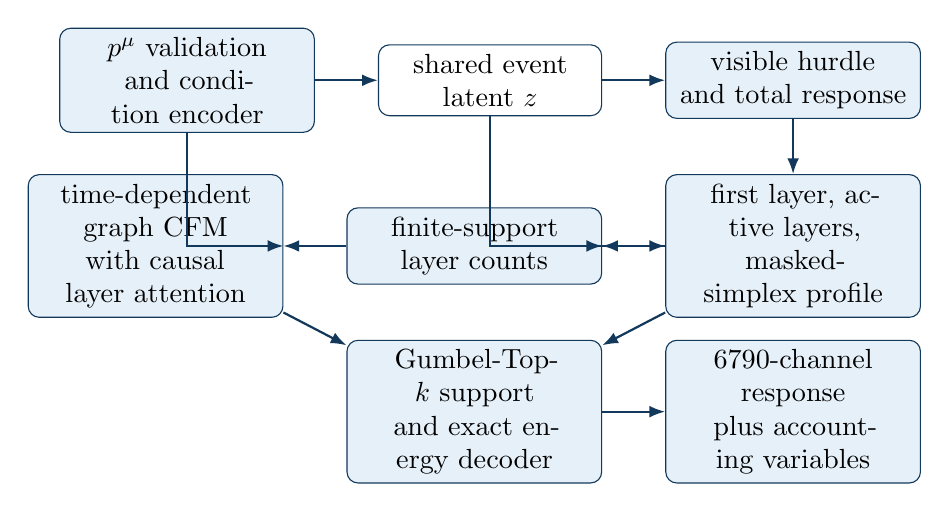
\begin{tikzpicture}[
  node distance=7mm and 8mm,
  box/.style={draw=deepblue,rounded corners,fill=lightblue,align=center,minimum height=9mm,text width=30mm},
  small/.style={draw=deepblue,rounded corners,fill=white,align=center,minimum height=8mm,text width=26mm},
  arr/.style={-{Latex[length=2mm]},thick,draw=deepblue}
]
\node[box] (p4) {$p^\mu$ validation\\and condition encoder};
\node[small,right=of p4] (latent) {shared event latent $z$};
\node[box,right=of latent] (response) {visible hurdle\\and total response};
\node[box,below=of response] (profile) {first layer, active layers,\\masked-simplex profile};
\node[box,left=of profile] (count) {finite-support\\layer counts};
\node[box,left=of count] (field) {time-dependent graph CFM\\with causal layer attention};
\node[box,below=of count] (decoder) {Gumbel-Top-$k$ support\\and exact energy decoder};
\node[box,right=of decoder] (out) {$6790$-channel response\\plus accounting variables};
\draw[arr] (p4)--(latent);
\draw[arr] (latent)--(response);
\draw[arr] (response)--(profile);
\draw[arr] (profile)--(count);
\draw[arr] (count)--(field);
\draw[arr] (field)--(decoder);
\draw[arr] (profile)--(decoder);
\draw[arr] (decoder)--(out);
\draw[arr] (latent) |- (profile);
\draw[arr] (latent) |- (count);
\draw[arr] (p4) |- (field);
\end{tikzpicture}
\caption{CBSC-ZDC factorization. All layer and cell outputs are generated conditionally on the same event condition and stochastic latent. The flow field updates all nodes in parallel at each solver step.}
\label{fig:architecture}
\end{figure}

\section{Longitudinal cascade model}

\subsection{Visible-response hurdle}
The event-level response point mass is
\begin{equation}
  V\sim\Bern(\pi_V(c,z)),\qquad \pi_V=\sigmoid(a_V(c,z)).
\end{equation}
When $V=0$, the modeled cell response, layer budgets, and counts are all zero. A separate no-response component is preferable to asking a continuous density to approximate a delta function at zero.

\subsection{Total response}
For the audited bounded mode, let $\rho=T/E\in(0,1)$. A flexible known choice is a finite mixture of beta distributions:
\begin{align}
  p(\rho\given V=1,c,z)
  &=\sum_{m=1}^{M}\pi_m(c,z)\,
  \BetaDist(\rho;\alpha_m(c,z),\beta_m(c,z)),\\
  \pi&=\softmax(a_\pi),\quad
  \alpha_m=\operatorname{softplus}(a_{\alpha,m})+\alpha_{\min},\\
  \beta_m&=\operatorname{softplus}(a_{\beta,m})+\beta_{\min},
  \qquad T=V E\rho.
  \label{eq:beta_mixture}
\end{align}
If the data have an endpoint mass at $\rho=1$, an explicit endpoint component should be added instead of relying on clipping.

\subsection{First-visible-layer survival model}
Let $h_\ell\in(0,1)$ denote a discrete hazard:
\begin{equation}
  h_\ell=p(S=\ell\given S\ge\ell,V=1,c,z,T).
\end{equation}
Then the unnormalized probability of starting at layer $\ell$ inside the detector is
\begin{equation}
  \tilde p_\ell=h_\ell\prod_{j<\ell}(1-h_j),
\end{equation}
and $p(S=\ell\given S<L)$ is obtained by normalizing $\tilde p_\ell$ across detector layers. This variable is the first \emph{visible} layer. It must not be described as the microscopic first nuclear interaction unless such truth is available.

\subsection{Exact active-layer support}
Conditional on $S$, the model generates $A_\ell\in\{0,1\}$ with
\begin{equation}
  A_\ell=0\quad(\ell<S),\qquad A_S=1.
\end{equation}
For $\ell>S$, activity may be generated by correlated Bernoulli logits conditioned on $(c,z,T,S)$, a causal discrete model, or a compact conditional flow over relaxed support variables followed by discrete sampling. The baseline implementation uses shared-latent Bernoulli logits and enforces the start constraints exactly. Because gaps can occur in sparse readout, the model should not force every post-start layer active unless the audited target supports that assumption.

\subsection{Masked-simplex energy allocation}
Let $q_0,\ldots,q_{L-1},q_{\mathrm{res}}$ be profile logits. Inactive layers receive $-\infty$ before normalization:
\begin{equation}
  \bar q_\ell=
  \begin{cases}
  q_\ell,&A_\ell=1,\\
  -\infty,&A_\ell=0.
  \end{cases}
\end{equation}
Define
\begin{equation}
  (w_0,\ldots,w_{L-1},w_{\mathrm{res}})
  =\softmax(\bar q_0,\ldots,\bar q_{L-1},q_{\mathrm{res}}),
\end{equation}
then
\begin{equation}
  D_\ell=T w_\ell,
  \qquad R_{\mathrm{res}}=T w_{\mathrm{res}}.
  \label{eq:simplex_profile}
\end{equation}
A logistic-normal profile is the reference sampler. A low-dimensional conditional flow-matching profile over the same masked-simplex target is a planned comparison, motivated by hierarchical calorimeter generators such as CaloFlow, iCaloFlow, L2LFlows, and CaloDREAM \citep{caloflow,icaloflow,l2lflows,convl2lflows,calodream}.

\begin{proposition}[Monotone remaining budget]
Assume $T\ge0$, $D_\ell\ge0$, and $\sum_{\ell=0}^{L-1}D_\ell+R_{\mathrm{res}}=T$. Define
\begin{equation}
  R_\ell=T-\sum_{j=0}^{\ell}D_j.
\end{equation}
Then $R_{\ell+1}\le R_\ell$ for every $\ell$, $R_\ell\ge R_{\mathrm{res}}\ge0$, and no ordering restriction is imposed on the individual $D_\ell$.
\end{proposition}
\begin{proof}
Since $D_{\ell+1}\ge0$,
$R_{\ell+1}=R_\ell-D_{\ell+1}\le R_\ell$.
Moreover,
$R_\ell=R_{\mathrm{res}}+\sum_{j>\ell}D_j\ge R_{\mathrm{res}}\ge0$.
The result contains no inequality comparing $D_{\ell+1}$ with $D_\ell$.
\end{proof}

\begin{remark}
The reserve is an accounting variable. Its scientific interpretation must be frozen: it may represent unmodeled/leakage response, subdetector-external energy, or simply a profile slack variable. It must not be called physical leakage without matching truth.
\end{remark}

\section{Finite-support count model}
For each layer $\ell$ with $N_\ell$ valid channels, generate
\begin{equation}
  K_\ell\sim\Cat(\eta_{\ell,0},\ldots,\eta_{\ell,N_\ell}),
  \label{eq:count_cat}
\end{equation}
where logits depend on $(c,z,D_\ell,A_\ell,\ell)$. A categorical count avoids the Poisson restriction $\operatorname{Var}(K)=\E[K]$ and permits exact masking of impossible values.

For thresholded mode, the resolved-count contract is piecewise:
\begin{equation}
K_\ell=
\begin{cases}
0, & 0\le D_\ell<\tau,\\
1,\ldots,\min\!\left(N_\ell,\left\lfloor D_\ell/\tau\right\rfloor\right),
& D_\ell\ge\tau.
\end{cases}
\label{eq:count_feasible}
\end{equation}
The first branch routes the layer budget to the recorded subthreshold residual rather than inventing a resolved cell. For raw-deposit mode, $K_\ell=0$ iff $D_\ell=0$, while $1\le K_\ell\le N_\ell$ whenever $D_\ell>0$. The count distribution is a central physics object, not an implementation detail, because exact support decoding transfers occupancy fidelity into the count model.

\section{Parallel conditional flow-matching spatial model}

\subsection{Why parallel rather than a 65-call rollout}
Layer-to-layer autoregression is a known and sometimes effective strategy \citep{icaloflow,l2lflows,convl2lflows}. For this detector it carries three risks: invalid index correspondence across irregular layers, accumulated free-running error, and serial latency. The proposed field updates all nodes at every numerical integration step, while causal layer attention and directed longitudinal graph edges preserve the intended dependence on earlier depth.

\subsection{Continuous target state}
The flow state has two channels per node:
\begin{equation}
  X_i=(s_i,r_i),
\end{equation}
where $s_i$ is a continuous support-ranking variable and $r_i$ is a positive-energy share variable. One supervised encoding is
\begin{align}
  s_i^*&=\logit\!\left(\varepsilon+(1-2\varepsilon)M_i\right),\\
  r_i^*&=M_i\left[\log(Y_i-\tau+\varepsilon)-
  \frac{1}{K_{\ell_i}}\sum_{j\in\mathcal S_{\ell_i}}
  \log(Y_j-\tau+\varepsilon)\right],
  \label{eq:state_encoding}
\end{align}
with $M_i=\ind\{i\in\mathcal S_{\ell_i}\}$. Equation~\eqref{eq:state_encoding} is evaluated only for layers with $K_{\ell_i}>0$; on zero-count layers set $r_i^*=0$ and omit the positive-share term from the loss. Other monotone encodings may be tested, but the decoder and target transform must be versioned together.

\subsection{Flow-matching objective}
Conditional flow matching learns a time-dependent velocity field without evaluating a simulation likelihood along an ODE path \citep{flowmatching,otcfm}. For a straight interpolation,
\begin{align}
  X_0&\sim\mathcal N(0,I),\qquad t\sim\mathcal U(0,1),\\
  X_t&=(1-t)X_0+tX_1,\\
  u_t&=X_1-X_0.
\end{align}
The vector field is
\begin{equation}
  v_\theta=v_\theta(X_t,t,c,z,\G,D,K),
\end{equation}
and the core loss is
\begin{equation}
  \mathcal L_{\mathrm{FM}}
  =\E\left[\left\|v_\theta(X_t,t,c,z,\G,D,K)-u_t\right\|_W^2\right],
  \label{eq:fm_loss}
\end{equation}
where $W$ may balance support and positive-share channels. The network must explicitly consume $t$; an implementation that accepts but ignores $t$ is not the specified field.

\subsection{Velocity network}
At each solver step:
\begin{enumerate}[leftmargin=2em]
  \item concatenate $X_t$ with static node features and layer-level dynamic features $\log(1+D_\ell)$ and $K_\ell/N_\ell$;
  \item add a learned time embedding and apply FiLM conditioning from $c$ and, if separate, $z$;
  \item apply edge-conditioned graph message passing using audited lateral and directed longitudinal edges;
  \item pool node states into layer tokens;
  \item apply a transformer with a causal layer mask, so layer $\ell$ attends only to layers $0,\ldots,\ell$;
  \item broadcast the mixed layer token to its nodes and predict the two velocity channels.
\end{enumerate}
This combines established graph, transformer, and conditional-flow components rather than proposing a new primitive \citep{calograph,calodream,calodiffusion}.

\subsection{Sampling}
Starting from $X(0)\sim\mathcal N(0,I)$, solve
\begin{equation}
  \frac{dX}{dt}=v_\theta(X,t,c,z,\G,D,K),\qquad t\in[0,1].
\end{equation}
Euler, midpoint, Heun, or an adaptive solver may be used. The solver, step count, precision, and random seed must be included in every timing and fidelity report. Published ZDC flow matching demonstrates that low-step and latent variants can achieve large speed gains on compact ALICE responses, but those numbers are not directly transferable to a 6,790-node detector \citep{fasterzdc,fasterzdc_code}.

\section{Exact sparsity and the anti-dust decoder}

\subsection{The failure mode}
A dense softmax allocation gives every valid cell positive energy. A model can then improve an aggregate energy loss by assigning a small value, such as $10^{-3}\GeV$, to many nominally empty cells. This can leave the total approximately correct while corrupting occupancy, positive-hit spectra, width, connectedness, and downstream reconstruction. Sparse HEP models explicitly show the value of modeling the point mass at zero \citep{sarm,calopointflow,caloclouds}. Calorimeter-flow studies also report that post-generation rescaling can lift nominally zero voxels and create excess low-energy hits \citep{icaloflow,convl2lflows}.

\subsection{Primary exact-support construction}
For layer $\ell$, let $B=D_\ell$ be the layer budget, $K=K_\ell$ the feasible count, $\mathcal I_\ell$ the valid channel set, and $a_i$ support logits. Select a subset $\mathcal S_\ell\subset\mathcal I_\ell$ with $|\mathcal S_\ell|=K$ by Gumbel-Top-$k$ sampling without replacement \citep{gumbeltopk}:
\begin{equation}
  \mathcal S_\ell=\operatorname{TopK}_{i\in\mathcal I_\ell}(a_i+g_i),
  \qquad g_i\sim\operatorname{Gumbel}(0,1).
  \label{eq:gumbel_topk}
\end{equation}
For selected-cell share logits $r_i$, define
\begin{equation}
  w_i=\frac{e^{r_i}}{\sum_{j\in\mathcal S_\ell}e^{r_j}},
  \qquad i\in\mathcal S_\ell.
\end{equation}
Decode
\begin{equation}
  \widehat Y_i=
  \begin{cases}
  \tau+(B-K\tau)w_i,&i\in\mathcal S_\ell,\\
  0,&i\notin\mathcal S_\ell,
  \end{cases}
  \label{eq:antidust_decoder}
\end{equation}
provided $B\ge K\tau$. If $B<\tau$, the feasible count is zero, every cell is zero, and $B$ is recorded as the layer-level subthreshold residual $U_\ell$.

\begin{theorem}[No-dust, exact-count, exact-budget decoder]
Consider a resolved layer with $B>0$ and an integer $K$ satisfying $1\le K\le N_\ell$ and $B\ge K\tau$. Let $\mathcal S_\ell$ have cardinality $K$, and let $w_i>0$ on $\mathcal S_\ell$ with $\sum_{i\in\mathcal S_\ell}w_i=1$. Then the decoder in \cref{eq:antidust_decoder} satisfies:
\begin{enumerate}[label=(\roman*),leftmargin=2em]
  \item $\widehat Y_i=0$ for $i\notin\mathcal S_\ell$;
  \item $\widehat Y_i\ge\tau$ for $i\in\mathcal S_\ell$;
  \item $\sum_{i\in\mathcal I_\ell}\widehat Y_i=B$;
  \item the number of positive cells is exactly $K$;
  \item no cell satisfies $0<\widehat Y_i<\tau$.
\end{enumerate}
For an unresolved thresholded layer with $0\le B<\tau$, define $K=0$, $\widehat Y_i=0$ for every cell, and $U_\ell=B$. For the zero-budget case in either target mode, define $K=0$, $\widehat Y_i=0$, and $U_\ell=0$.
\end{theorem}
\begin{proof}
Items (i) and (ii) follow directly from the piecewise definition and $B-K\tau\ge0$. For (iii),
\begin{equation}
  \sum_i\widehat Y_i
  =K\tau+(B-K\tau)\sum_{i\in\mathcal S_\ell}w_i=B.
\end{equation}
Because $K\ge1$ and every selected weight is positive, exactly the $K$ selected cells are positive. Item (v) follows because each cell is either zero or at least $\tau$. The residual case is the stated definition.
\end{proof}

\begin{corollary}[Event accounting]
If each layer is decoded as above, then
\begin{equation}
  \sum_{i=1}^{N}\widehat Y_i+\sum_{\ell=0}^{L-1}U_\ell+R_{\mathrm{res}}=T.
  \label{eq:event_accounting}
\end{equation}
\end{corollary}

\subsection{What exact \texorpdfstring{Top-$k$}{Top-k} does not guarantee}
The decoder guarantees exact support \emph{conditional on the generated count}. It cannot prevent a poorly trained count network from requesting too many cells. In particular, a model could choose $K_\ell=N_\ell$ and remain algebraically valid while producing physically incorrect occupancy. The experiment therefore trains and reports the count as an independent random variable. For a frozen target threshold,
\begin{equation}
  K_\ell^{*}=\sum_{i:\ell_i=\ell}\ind\{Y_i\ge\tau\}
\end{equation}
(with strict positivity replacing $Y_i\ge\tau$ when $\tau=0$), and $p_\theta(K_\ell\mid c,z,D_\ell,A_\ell)$ is optimized by categorical negative log-likelihood. Requested-count calibration, realized-count calibration, and occupancy distributions are reported separately from the total loss. Support logits are supervised or ranked against the corresponding truth set. Later training exposes the spatial field to generated counts and generated support so that good truth-conditioned behavior cannot conceal free-running support errors. Thus Top-$k$ removes dense low-energy dust, while the count and support objectives prevent the model from evading that constraint by declaring every cell active.

\subsection{Training the discrete support}
Hard Top-$k$ is non-differentiable through the selected indices. It is therefore the exact sampling and evaluation decoder, not by itself a complete training objective. Recommended known options are:
\begin{enumerate}[leftmargin=2em]
  \item supervise support logits with class-balanced binary cross entropy or ranking loss while training positive shares on truth support;
  \item use a continuous subset relaxation or straight-through estimator during joint fine-tuning \citep{relaxedsubset};
  \item expose the positive-share model to generated counts and generated support during later stages to reduce truth-mask/sample-mask mismatch;
  \item compare exact Top-$k$ with sparsemax/entmax and hard-concrete gates \citep{sparsemax,entmax,hardconcrete}.
\end{enumerate}
The primary specification retains Top-$k$ because its support size, zeros, and accounting are directly auditable. The alternatives are ablations, not assumed upgrades.

\section{Training objectives}
The complete objective is modular:
\begin{align}
\mathcal L
&=\lambda_V\mathcal L_V
 +\lambda_\rho\mathcal L_\rho
 +\lambda_S\mathcal L_S
 +\lambda_A\mathcal L_A
 +\lambda_D\mathcal L_D
 +\lambda_K\mathcal L_K \nonumber\\
&\quad+\lambda_{\mathrm{FM}}\mathcal L_{\mathrm{FM}}
 +\lambda_{\mathrm{sup}}\mathcal L_{\mathrm{sup}}
 +\lambda_{\mathrm{aux}}\mathcal L_{\mathrm{aux}}.
\end{align}
The terms are:
\begin{align}
  \mathcal L_V&=\operatorname{BCE}(V,\pi_V),\\
  \mathcal L_\rho&=-\log p(\rho\given V=1,c,z),\\
  \mathcal L_S&=-\log p(S\given V=1,c,z,T),\\
  \mathcal L_A&=\operatorname{BCE}(A,\pi_A)\text{ on allowed layers},\\
  \mathcal L_K&=\sum_\ell\operatorname{CE}(K_\ell,\eta_\ell),\\
  \mathcal L_{\mathrm{sup}}&=\operatorname{BCE}(M,\sigma(s))\text{ or a ranking/relaxed-set loss}.
\end{align}
$\mathcal L_D$ may be a masked-simplex likelihood, profile flow-matching loss, or a set of conditional distributional terms. $\mathcal L_{\mathrm{aux}}$ may include moment or positive-hit-spectrum diagnostics, but it must not reduce the experiment to eventwise regression against an arbitrary independent Geant4 shower.

All unweighted component losses, weighted contributions, and stage-wise gradient norms should be reported. Loss weights should be selected on a frozen validation protocol, not tuned against the final test set. A lower scalar loss is not sufficient evidence of improved FastMC fidelity; the previous HGF-ZDC run supplied a direct counterexample \citep{project_hgf_audit}.

\section{Data pipeline and provenance}

\subsection{Raw ROOT audit}
Before model training, the converter should report:
\begin{enumerate}[leftmargin=2em]
  \item file hashes, ROOT tree name, branch names, types, units, and entry counts;
  \item four-momentum mass-shell residuals and energy/angular support;
  \item exact channel-ID decoding, duplicate IDs, invalid IDs, sentinel records, and energy carried by excluded records;
  \item agreement between reconstructed ECAL/HCAL totals and producer summary branches;
  \item zero-response frequency, total-response support, layer occupancy, and threshold sensitivity;
  \item fixed versus variable gun vertex and the implied condition manifold;
  \item available job, run, event, and random-seed provenance for leakage-safe splitting.
\end{enumerate}
The small attached ROOT file has the same branch structure but a different Geant4 run and must be used only as a schema/reference fixture. In the current execution environment, ROOT/Uproot/Awkward were not available for a fresh numerical decode; the repository therefore contains a branch-map-oriented adapter scaffold rather than fabricated event statistics.

\subsection{Canonical tensors}
A canonical event contains at least:
\begin{lstlisting}
p4                 float32 [4]
cell_energy_raw    float32 [6790]
cell_energy_tau    float32 [6790]   # only in thresholded mode
layer_energy       float32 [65]
layer_hit_count    int64   [65]
active_layer       bool    [65]
first_visible      int64
subthreshold       float32 [65]     # thresholded mode
metadata           event/run/source provenance
\end{lstlisting}
Channel order and geometry version must be immutable and hashed. Padding must not be confused with valid zero-energy cells.

\subsection{Splitting}
The preferred split unit is an independent Geant4 generation group, such as job/run/seed family. If no grouping metadata exist, a deterministic row-index hash split may be unavoidable, but its limitation must be reported and duplicate/correlation searches should be performed. All data-derived normalization, thresholds, mixture initialization, and model selection use training and validation data only. The final test manifest is read only for the final declared evaluation.

\subsection{Training range experiment}
Run two matched experiments:
\begin{enumerate}[label=\textbf{R\arabic*.},leftmargin=2em]
  \item train on $50$--$250\GeV$ only;
  \item train on the full supported $0$--$300\GeV$ range while retaining the same architecture and primary reporting domain.
\end{enumerate}
Broader support may reduce boundary artifacts but may also consume capacity on qualitatively different low-energy response. The effect must be measured rather than assumed. This has no direct relationship to collider event pileup: training on a wider single-neutron energy range does not itself teach superposition of multiple particles. A pileup-capable model would require multi-particle conditioning or a validated composition procedure.

\section{Staged implementation and Vertex AI execution plan}

\subsection{Stage sequence}
The recommended sequence is:
\begin{longtable}{p{0.09\textwidth}p{0.33\textwidth}p{0.50\textwidth}}
\toprule
Stage & Work & Recommended report \\
\midrule
\endfirsthead
\toprule
Stage & Work & Recommended report \\
\midrule
\endhead
0 & Freeze target, threshold, geometry, split, and provenance. & Data-contract report with hashes, branch map, support plots, sentinel accounting, and condition-manifold statement. \\
1 & Train visible hurdle and total-response model. & Conditional zero rate, response quantiles, means, variances, tails, calibration, and train/validation uncertainty. \\
2 & Train first-visible, active-layer, and masked-simplex profile. & Start-depth distribution, per-layer zero rate, energy profiles, cumulative profiles, late energy, and covariance. \\
3 & Train finite-support count model. & Count calibration and distributions by energy, angle, layer, start depth, and layer budget. \\
4 & Train spatial CFM using truth profile and truth counts. & Time-dependent loss, support ranking, positive-hit spectrum, geometry-aware morphology, memory, and throughput. \\
5 & Expose spatial model to generated counts/support and generated profile. & Difference between truth-conditioned and free-running results; support mismatch and error propagation. \\
6 & Optional joint fine-tuning. & All component losses and gradients plus full-cascade free-running metrics. \\
7 & Baselines and ablations. & Matched data, optimization steps, hardware, precision, solver, parameters, memory, and wall time. \\
8 & Final held-out and downstream study. & Primary-domain, stress-domain, reconstruction, uncertainty, and timing reports kept separate. \\
\bottomrule
\end{longtable}
These are reporting locations, not user-imposed pass/fail gates. Algebraic assertions such as finite tensors and exact accounting remain software invariants because violating them means the implementation no longer matches the specification.

\subsection{Vertex job layout}
Each Vertex job should be immutable and self-describing:
\begin{lstlisting}
runs/<experiment_id>/
  config_resolved.yaml
  environment.txt
  git_commit.txt
  data_manifest.json
  geometry_hash.txt
  statistics.pt
  checkpoints/
  histories/
  free_running_validation/
  timing/
  logs/
\end{lstlisting}
Use checkpoint resume with optimizer, scheduler, scaler, random-number-generator states, epoch/step counters, and validation-bank version. Periodic checkpoint upload should write only changed artifacts rather than resynchronizing the complete output tree.

\subsection{Precision and performance}
Begin with float32 accumulation in graph reductions and profile/accounting operations. Mixed precision is introduced only after finite-gradient and output-equivalence probes, because earlier project work found several graph/autocast dtype and accumulation failures \citep{project_hgf_audit}. Report model-only and end-to-end timing separately at batch 1 and representative larger batches.

\section{Baselines and controlled comparisons}

\subsection{Direct ZDC references}
The following repositories are the highest-priority external comparisons:
\begin{enumerate}[leftmargin=2em]
  \item \code{m-wojnar/faster\_zdc}: full and latent flow-matching models accompanying the ALICE ZN/ZP study \citep{fasterzdc,fasterzdc_code};
  \item \code{m-wojnar/zdc}: VAE, GAN, vector-quantized, and diffusion-era ALICE ZDC work \citep{zdc_code,zdcmachinelearning,zdcdiffusion};
  \item ExpertSim's mixture-of-generative-experts implementation for heterogeneous ZDC responses \citep{expertsim};
  \item the inverse-autoregressive-flow ZDC line, where code availability and license must be confirmed before integration \citep{zdc_iaf}.
\end{enumerate}
These should first be reproduced on their native representations. Any adaptation to 6,790 irregular channels is a new experiment and must not be called a direct reproduction.

\subsection{Internal matched baseline ladder}
On the identical training/validation manifests, optimization steps, solver steps, precision, and hardware, compare:
\begin{description}[leftmargin=2.3em,style=nextline]
  \item[B0: conditional empirical/template baseline] A non-neural or low-capacity model for visible probability, total response, profile, count, and an entry-centered spatial template with empirical residuals.
  \item[B1: non-graph parallel CFM] Same profile, count, state encoding, and exact decoder as CBSC-ZDC; remove graph message passing and retain only node features/layer tokens.
  \item[M1: mixture-of-experts] Route broad response regimes to specialized versions of a compact known generator, motivated by ExpertSim \citep{expertsim}.
  \item[G1: CBSC-ZDC] Full graph plus causal layer attention.
  \item[S1: single-stage graph flow] The supplied baseline that removes the start/profile hierarchy and learns the full response in one graph flow \citep{project_single_stage}.
  \item[A1: serial previous-layer model] A diagnostic layer-autoregressive ablation using valid geometric correspondence; included to measure fidelity/latency, not assumed superior.
  \item[P1: sparse point-cloud model] Optional comparison if the hit threshold and readout mapping are frozen, motivated by CaloClouds and CaloPointFlow \citep{caloclouds,caloclouds2,calopointflow}.
\end{description}
The graph is justified only if it improves predeclared geometry-sensitive results enough to compensate for its latency and memory. Production fast simulation is often hybrid rather than architecturally pure; AtlFast3 is an important precedent \citep{atlfast3}.

\section{Recommended QA and reporting}

\subsection{Software and algebraic QA}
At construction and sampling, report or assert:
\begin{itemize}[leftmargin=2em]
  \item tensor shapes, dtypes, devices, masks, and edge ranges;
  \item no NaN or infinity and no negative cell energy;
  \item zero energy in invalid or padded channels;
  \item exact support-count equality;
  \item zero forbidden dust cells $0<Y_i<\tau$ in thresholded mode;
  \item per-layer equality between resolved cell energy and $D_\ell-U_\ell$;
  \item event identity in \cref{eq:event_accounting};
  \item $T\le E$ only when the bounded raw-deposit assumption has been audited;
  \item deterministic replay under fixed seeds and diversity under different seeds;
  \item explicit dependence of the velocity field on flow time $t$.
\end{itemize}

\subsection{Training-time monitoring}
A frozen validation bank should be generated in free-running mode during training. Report:
\begin{enumerate}[leftmargin=2em]
  \item all component losses and stage-wise gradient norms;
  \item total-response mean, width, quantiles, and zero rate by condition;
  \item first-visible layer, active-layer count, longitudinal profile, and late-energy fraction;
  \item hit count, positive-hit spectrum, cell occupancy, and subthreshold residual;
  \item transverse centroid, RMS, $R_{50}$, $R_{90}$, maximum-cell and top-$k$ fractions;
  \item correlations among response, start depth, hit count, width, ECAL fraction, and late energy;
  \item inference time, memory, and numerical failures.
\end{enumerate}
A checkpoint is not described as improving merely because the training loss decreases. Report paired/bootstrap uncertainty for differences between checkpoints and label the result as improvement, plateau, regression, or inconclusive according to the frozen analysis plan.

\subsection{Distributional evaluation}
Use complementary diagnostics rather than one aggregate distance:
\begin{itemize}[leftmargin=2em]
  \item one-dimensional conditional histograms and distances for named physics observables;
  \item high-level classifier two-sample tests;
  \item geometry-aware low-level graph, sparse, or point-cloud classifiers;
  \item Fr\'echet and kernel physics distances with a frozen disclosed feature extractor \citep{hepgenerative_metrics};
  \item precision/recall or coverage diagnostics to distinguish realistic but incomplete generation from broad unphysical generation \citep{precisionrecall,improvedpr};
  \item nearest-neighbor train/test comparisons for memorization;
  \item truth-half versus truth-half statistical floors;
  \item repeated-condition Geant4 and FastMC ensembles for conditional variance and tails.
\end{itemize}
Averaging an independent per-cell distance over thousands of mostly zero channels is not sufficient evidence of joint spatial closure.

\subsection{Downstream and amplification studies}
Freeze the reconstruction model before comparing Geant4 and FastMC. Report reconstructed energy scale/resolution, position/angle resolution, efficiencies, threshold behavior, and tail migration. Also perform train-on-Geant4/test-on-FastMC and train-on-FastMC/test-on-locked-Geant4 studies. Recent work emphasizes that full-physics reconstruction benchmarks can reveal failures hidden by shower-image metrics \citep{fullphysicsbenchmark}.

Generating many more FastMC events than training events reduces sampling noise but not surrogate bias. Any ``calomplification'' claim must be observable-specific and measured against an independent larger Geant4 reference \citep{calomplification}.

\section{Failure modes and required interpretations}

\begin{longtable}{p{0.25\textwidth}p{0.31\textwidth}p{0.35\textwidth}}
\toprule
Failure mode & Symptom & Required diagnosis or mitigation \\
\midrule
\endfirsthead
\toprule
Failure mode & Symptom & Required diagnosis or mitigation \\
\midrule
\endhead
Dense energy dust & Many cells contain tiny positive values; occupancy and width inflate. & Exact count/support decoder; threshold contract; positive-hit and subthreshold reports. \\
Unbounded response tail & Rare samples dominate the mean or exceed physically audited support. & Target-correct response distribution; profile-only million-sample tail audit. \\
Profile underweighting & Global flow loss improves while response bias stays fixed. & Separate response objective/gradients; standalone response model; truth-profile cross-tests. \\
Mode averaging & Correct pooled mean, wrong zero/late/leakage regimes. & Hurdle and mixture routing; conditional precision/recall; repeated conditions. \\
Count bottleneck & Exact decoder produces wrong morphology because $K_\ell$ is wrong. & Count calibration; truth-count versus generated-count spatial tests; compare sparse alternatives. \\
Exposure bias & Truth-conditioned stage is good, full cascade degrades. & Generated-condition exposure, cross-combination matrix, optional joint fine-tuning. \\
Invalid graph & Isolated valid nodes or readout-index edges. & Geometry audit, degree/connectivity report, physical edge provenance, no-graph comparison. \\
Condition ignorance & Pooled samples look plausible but anchors do not change with $p^\mu$. & Condition permutation, local interpolation, repeated-p4 evaluation. \\
Support extrapolation & Edge or angle claims outside Geant4 coverage. & Report as stress/OOD; generate new anchored Geant4 data. \\
Latency failure & Graph/ODE model is slower than useful alternatives. & Profile every stage; solver sweep; distillation/latent comparison only after fidelity teacher exists. \\
\bottomrule
\end{longtable}

\section{Implementation contract}

\subsection{Reference tensor interface}
\begin{longtable}{p{0.27\textwidth}p{0.22\textwidth}p{0.42\textwidth}}
\toprule
Object & Shape & Contract \\
\midrule
\endfirsthead
\toprule
Object & Shape & Contract \\
\midrule
\endhead
$p^\mu$ & $[B,4]$ & Raw condition in GeV; neutron mass-shell validated. \\
Condition embedding $c$ & $[B,C]$ & Derived only from $p^\mu$. \\
Node features & $[6790,F_n]$ & Static geometry; versioned and hashed. \\
Edge index & $[2,N_e]$ & Static valid node IDs; edge direction/type documented. \\
Edge features & $[N_e,F_e]$ & Relative displacement, distance, overlap/type encodings. \\
Layer index & $[6790]$ & Integer in $[0,64]$. \\
Profile budgets $D$ & $[B,65]$ & Nonnegative; zero on inactive layers. \\
Counts $K$ & $[B,65]$ & Integer and feasible by geometry/threshold. \\
Flow state $X_t$ & $[B,6790,2]$ & Support-ranking and share channels. \\
Final cell energy $Y$ & $[B,6790]$ & Nonnegative, exact zeros outside support. \\
Residual $U$ & $[B,65]$ & Subthreshold energy in thresholded mode. \\
Reserve & $[B,1]$ & Profile accounting channel with frozen interpretation. \\
\bottomrule
\end{longtable}

\subsection{Reference hyperparameters for the first pilot}
These are starting values for a matched pilot, not empirically established optima:
\begin{center}
\begin{tabular}{ll}
\toprule
Component & Initial specification \\
\midrule
Condition embedding & $C=128$, residual MLP, SiLU, LayerNorm \\
Shared latent & $32$ Gaussian dimensions \\
Response mixture & $4$ beta components plus visible hurdle \\
Profile network & hidden $256$; logistic-normal or low-dimensional CFM \\
Count network & hidden $192$; categorical support $0,\ldots,N_\ell$ \\
Spatial hidden width & $96$ \\
Graph blocks & $2$ edge-conditioned residual blocks \\
Layer transformer & $3$ blocks, $4$ heads, causal mask \\
Flow solver & compare $4$, $8$, and $16$ evaluations \\
Primary state & two channels per node \\
Support sampling & stochastic Gumbel-Top-$k$; deterministic Top-$k$ for diagnostics \\
Precision & float32 reference; mixed precision only after equivalence tests \\
Pilot data & matched $50$k--$100$k-event studies \\
\bottomrule
\end{tabular}
\end{center}

\subsection{Pseudocode}
\begin{lstlisting}
function SAMPLE(p4, geometry, seed):
    validate_units_shape_mass_shell(p4)
    c = condition_encoder(minimal_features(p4))
    z = Normal(0, I).sample(seed)

    V = sample_visible(c, z)
    rho = sample_target_correct_response(c, z, V)
    T = incident_energy(p4) * rho

    S = sample_first_visible_layer(c, z, T, V)
    A = sample_active_layers(c, z, T, S, V)
    D, reserve = sample_masked_simplex_profile(c, z, T, A)
    K = sample_feasible_layer_counts(c, z, D, A, threshold)

    X = Normal(0, I).sample(seed)
    for solver_time in configured_grid:
        velocity = spatial_graph_field(
            X, solver_time, c, geometry, D, K
        )
        X = solver_step(X, velocity)

    support = gumbel_topk(X.support_scores, K, geometry.valid)
    Y, residual = exact_threshold_safe_decode(
        support, X.share_scores, D, K, threshold
    )
    assert_structural_invariants(Y, residual, reserve, T)
    return Y, diagnostics
\end{lstlisting}

\section{Software QA status of the supplied scaffold}
The revised repository is an executable reference scaffold, not a full Vertex training system. Static compilation and unit tests currently exercise:
\begin{itemize}[leftmargin=2em]
  \item bounded response and exact profile accounting;
  \item first-visible-layer/start-support consistency;
  \item vectorized exact-$K$ support decoding;
  \item no forbidden threshold dust and correct subthreshold residuals;
  \item valid-mask handling;
  \item time dependence of the flow field;
  \item edge-conditioned message passing and invalid-edge rejection;
  \item end-to-end sampling identities on synthetic geometry;
  \item fixed-seed replay.
\end{itemize}
The latest local command result is \code{30 passed}; measured source-and-test statement/branch coverage is 100\% under the synthetic unit suite. PyTorch reports a nested-tensor optimization warning caused by the transformer's \code{norm\_first=True}. The warning does not indicate a numerical failure, but the production timing study should profile alternative transformer settings. Coverage demonstrates execution of the current scaffold paths, not fidelity to Geant4.

The hard decoder is vectorized by layer but remains an inference/evaluation operation. A production training entry point, ROOT branch map, canonical converter, distributed data loader, geometry builder, complete loss orchestration, Vertex launcher, and full evaluation package remain implementation work. This distinction is stated to prevent a tested scaffold from being misrepresented as a trained simulator.

\section{Research literature audit and evidence depth}
A prior project catalogue contains 600 linked works and a separate survey contains more than 100 named model instances. They are retained as broad discovery and contribution maps. They are not represented here as 600 line-by-line full-text peer reviews. The present specification relies on a smaller core bibliography whose claims were checked against primary papers, official documentation, or project evidence. The supplementary catalogue marks evidence depth, and auditors should not treat title/abstract or bibliography screening as equivalent to full-paper replication.

The broad survey nevertheless supports several robust synthesis points: there is no universal winner across CaloChallenge datasets and metrics; hierarchical global-to-local designs recur across successful flows and flow-matching models; diffusion and score models often offer high fidelity but require sampling acceleration; GANs are fast but vulnerable to coverage failure; point-cloud and sparse models directly address empty-cell inefficiency; mixtures are relevant to heterogeneous ZDC responses; and production fast simulation is commonly hybrid \citep{calochallenge,caloflow2,calodream,calodiffusion,caloscore2,caloclouds2,expertsim,atlfast3}.

\section{Five-minute explanation for a general science-fair judge}
Detailed particle simulations are accurate but expensive because they track many random interactions through matter. This project asks whether a neural network can learn the distribution of what a neutron leaves in a forward calorimeter without retracing every microscopic step.

The detector is divided into thousands of readout cells and many depth layers. The model receives only the neutron's energy and direction through its four-momentum. It first decides whether a visible shower occurs, how much total energy appears, where the shower begins, how that energy is shared across depth, and how many cells are active. A final generative model draws the detailed pattern.

The main physics correction is that energy in successive layers does not always decrease. A neutron can travel some distance before colliding, so the shower can start late and grow. What must decrease is the amount of energy still available to allocate. The model enforces that accounting exactly.

The model also prevents a common machine-learning shortcut. A network might put a tiny amount of energy into every cell to reduce its average error. Here it must first choose an exact number of hit cells; all other cells are exactly zero. The selected cells share the layer's energy exactly. This makes the output auditable.

The test is not whether the images look convincing. The model will be compared with held-out Geant4 simulations on total response, shower depth, width, occupancy, rare tails, correlations, downstream reconstruction, and speed. Several published ZDC and calorimeter models will be run as baselines. The result may show that the proposed hierarchy helps, or that a simpler flow is better. Either outcome is scientifically useful because the comparison is controlled and falsifiable.

\section{Five-minute explanation for a computational HEP physicist}
The target is a conditional readout-level density $\pG(Y\mid p^\mu,\G)$ for single neutrons, with 6,790 nonnegative channels across one ECAL and 64 HCAL layers. The only raw event condition is $p^\mu$; geometry is static. The proposal is a known-component hierarchy designed around previously observed structural failures.

A visible-response hurdle precedes a target-audited total-response density, initially a beta mixture for $\rho=T/E$. A discrete survival model generates first visible depth. A correlated layer mask creates exact zero layers, and a masked simplex allocates $T$ over active layers plus an accounting reserve. This makes the residual budget monotone without imposing the unphysical constraint $D_{\ell+1}\le D_\ell$.

Counts are categorical with exact geometry- and threshold-feasibility masks. The spatial generator is a time-dependent CFM field on two node channels, conditioned on profile and counts. Each solver step applies edge-conditioned message passing and a causal layer-token transformer, updating all nodes in parallel. This replaces a serial 65-layer rollout while retaining longitudinal context.

At sampling, Gumbel-Top-$k$ selects exactly $K_\ell$ cells. For a frozen threshold $\tau$, selected energies are
$\tau+(D_\ell-K_\ell\tau)\softmax(r)$; unselected cells are zero. If $D_\ell<\tau$, the budget becomes a layer residual rather than voxel dust. The decoder proves exact count, threshold consistency, and energy closure. Training uses supervised/relaxed support objectives because hard Top-$k$ is not differentiable.

The experiment separates profile-only, truth-profile spatial, generated-profile spatial, and full-cascade evaluations. Required comparisons are a competent empirical baseline, a matched non-graph CFM, a response-regime mixture, the full graph model, the supplied single-stage graph flow, a valid serial ablation, and direct reproduction of published ALICE ZDC repositories on native data. No architecture is promoted by loss alone; free-running conditional distributions, geometry-aware C2ST, physics distances, coverage, reconstruction closure, and matched timing are reported. The specification guarantees structural validity under the target assumptions, not Geant4 fidelity.

\section{Conclusions}
The proposed experiment is worth implementing. Its defensible content is not a new neural primitive but a detector-specific synthesis of established ideas with exact contracts. The original monotone layer-deposit concept is replaced by monotone residual accounting. Exact layer support and finite counts prevent dense positive profiles. A threshold-safe Top-$k$ decoder prevents artificial low-energy dust. Parallel graph-conditioned flow matching preserves longitudinal dependence without a serial rollout. The only raw condition remains four-momentum.

If implemented exactly, with a verified ROOT/geometry/target contract and the stated baseline comparisons, the project should yield a valid academic answer to whether this combination improves the speed--fidelity frontier for neutron ZDC simulation. A negative result would remain informative: it could show that the hierarchy, graph, exact count, or wider training range does not earn its complexity. What cannot be promised in advance is numerical agreement with Geant4. That must be established by the experiment.

\appendix
\section{Claim-to-evidence map}
\begin{longtable}{p{0.34\textwidth}p{0.56\textwidth}}
\toprule
Claim & Evidence or status \\
\midrule
\endfirsthead
\toprule
Claim & Evidence or status \\
\midrule
\endhead
Geant4 hadronic interactions are stochastic and model/cross-section dependent. & Geant4 toolkit papers and official hadronic physics manual \citep{geant4_2003,geant4_2016,geant4_hadronic_manual}. \\
Neutron hadronic layer deposits need not decrease monotonically. & General hadronic-shower physics and longitudinal parameterization literature \citep{hadronic_profile}; follows also from stochastic first interaction and cascade development. \\
ZDC response is detector-specific. & ALICE TDR and multinucleon/ZDC performance study \citep{alice_zdc_tdr,zdc_multinucleon}. \\
Hierarchical global/layer/local generation is established. & CaloFlow, iCaloFlow, L2LFlows, CaloDREAM \citep{caloflow,icaloflow,l2lflows,calodream}. \\
Conditional flow matching is an established training framework. & Flow Matching and minibatch OT-CFM \citep{flowmatching,otcfm}. \\
Sparse exact-support modeling addresses empty-cell structure. & SARM, CaloPointFlow, CaloClouds \citep{sarm,calopointflow,caloclouds}. \\
Gumbel-Top-$k$ samples a fixed-size subset without replacement. & Kool et al. \citep{gumbeltopk}. \\
Sparsemax, entmax, hard-concrete, and relaxed subset methods are known alternatives. & \citep{sparsemax,entmax,hardconcrete,relaxedsubset}. \\
Published ALICE ZDC FM is a direct methodological baseline. & Wojnar paper and repository \citep{fasterzdc,fasterzdc_code}. \\
Mixtures are relevant to heterogeneous ZDC response. & ExpertSim \citep{expertsim}. \\
Prior project models had documented structural and evaluation failures. & Internal independent audits \citep{project_legacy_audit,project_hgf_audit}. \\
Exact decoder invariants hold. & Proved in this document and covered by synthetic unit tests; no external empirical claim. \\
CBSC-ZDC reproduces Geant4. & Not claimed; requires training and held-out evaluation. \\
\bottomrule
\end{longtable}

\section{Chronological design corrections}
\begin{enumerate}[leftmargin=2em]
  \item Rejected monotone per-layer deposits after reviewing neutron/hadronic shower physics.
  \item Retained monotone remaining-budget accounting, then replaced long multiplicative stick breaking with exact active support and masked-simplex allocation to avoid depth-order pressure.
  \item Separated no-response, total response, first-visible depth, active layers, counts, and spatial allocation.
  \item Corrected the spatial scaffold so the velocity field explicitly depends on flow time.
  \item Added valid-node masking and edge-conditioned graph message passing with range checks.
  \item Replaced nested event/layer support decoding with a layer-vectorized exact-$K$ implementation.
  \item Added first-visible-layer survival semantics and enforced zero activity before the sampled start.
  \item Added the anti-dust threshold/residual contract and proved its invariants.
  \item Clarified that hard Top-$k$ is an inference/evaluation decoder and needs supervised or relaxed support training.
  \item Separated structural correctness from empirical fidelity and removed any suggestion that unit tests validate the simulator.
  \item Reclassified the 600-work catalogue as a discovery/contribution map rather than 600 full-text replications.
\end{enumerate}
The repository's chronological audit log records these externalized research and engineering decisions without purporting to reveal private internal reasoning.

\section{Recommended auditor checklist}
\begin{enumerate}[leftmargin=2em]
  \item Confirm the ROOT branch map, units, channel codec, sentinel meaning, and event counts.
  \item Confirm that the target is raw deposit or thresholded readout, not a mixture of conventions.
  \item Confirm the energy-support assumption before enabling $T/E\le1$.
  \item Confirm geometry hashes and that every valid node has appropriate adjacency or is intentionally isolated.
  \item Confirm the sole raw condition is $p^\mu$ and that any entry coordinate is deterministic under a fixed vertex.
  \item Re-run static compilation, unit tests, and deterministic replay.
  \item Trace every generated tensor to the mathematical variable defined in this paper.
  \item Confirm that the flow field consumes $t$ and that the solver is documented.
  \item Confirm that hard support is not the only gradient path during training.
  \item Confirm zero dust, exact count, per-layer accounting, and event accounting on a large generated sample.
  \item Confirm primary-domain and stress-domain reports are separate.
  \item Confirm the single-stage, no-graph, mixture, empirical, and external ZDC comparisons are matched or their mismatches disclosed.
  \item Confirm the final test set was not used for preprocessing, threshold choice, or checkpoint selection.
  \item Confirm every speed comparison reports hardware, batch, precision, steps, preprocessing, and output dimensionality.
  \item Confirm conclusions do not exceed statistical precision or the supported condition manifold.
\end{enumerate}

\printbibliography[title={References}]

\end{document}
